\chapter{Implementation and Evaluation}
\label{Implementation_and_Evaluation}
In this chapter, we evaluate the methods presented in Chapter 3. First, the environment and the reason of using them will be explained. Then, we will show different experiments and their corresponding results.

\section{General setup}
Table~~\ref{table:Experiment_table} is a summary of all the tools and their versions in the evaluation. We use Mininet to simulate the data center network \cite{Mininet}. It allows us to creates a large-scale virtual network easily. It provides Python APIs as well as a command line interface to customize the network. It also offers an interactive interface to test the connectivity and performance.

\begin{table}[H]
\centering
\caption{Experimental environment summary}
\begin{tabular}{|l|p{4cm}|p{4.5cm}}
\hline Item & Detail version \\
\hline
\hline Operating system & Ubuntu 14.04 x86\_64 \\
\hline Controller & Ryu\_manager 4.0 \\
\hline Network Emulator & Mininet 2.2.1 \\
\hline Topology generator & Fast Network Simulation Setup (FNSS) 0.6.1\\
\hline Packet Generator & Ryu packet library API \\
\hline Southbound API & OpenFlow 1.3 \\
\hline Virtual switch & OpenvSwitch 2.5.0 \\
\hline 
\end{tabular}
\label{table:Experiment_table}
\end{table}

To evaluate the effectiveness of the detection method under various scenarios, there will be XXXX network topologies in the evaluation. They are generated by Fast Network Simulation Setup (FNSS), a Python module able to generate various types of network topology. It not only supports DCN topologies, but also provides the Mininet API, making it extremely easy to import the generated topology into Mininet. The network topologies we use are two-tier topology, three-tier topology and fat-tree topology of various sizes. The details including number of switches and average degree (i.e. the number of links between two switches) are shown in Table~\ref{table:network_env}. The numbers in the topology name are parameters such as number of core switches, aggregation switches or edge switches, which characterize the network size. These parameters have the same meaning as the ones in \cite{FNSS}.

\begin{table}[H]
\centering
\caption{Details of network topologies}
\begin{tabular}{|l||l|l|l|}
\hline topology type & number of switches & average degree \\
\hline
\hline fat\_tree\_2 & 5 & 2 \\
\hline fat\_tree\_4 & 20 & 4 \\
\hline fat\_tree\_6 & 45 & 6 \\
\hline fat\_tree\_8 & 80 & 8 \\
\hline fat\_tree\_10 & 125 & 10 \\
\hline 
\hline two\_tier\_2\_3 & 5 & 3 \\
\hline two\_tier\_3\_4 & 7 & 4 \\
\hline two\_tier\_4\_4 & 8 & 4.5 \\
\hline two\_tier\_5\_4 & 9 & 4.8 \\
\hline two\_tier\_6\_8 & 14 & 7.42 \\
\hline two\_tier\_6\_14 & 20 & 9.1 \\
\hline two\_tier\_8\_10 & 18 & 9.4 \\
\hline two\_tier\_10\_10 & 20 & 10.5 \\
\hline two\_tier\_12\_8 & 20 & 10 \\
\hline two\_tier\_12\_12 & 24 & 12.5 \\
\hline two\_tier\_14\_6 & 20 & 8.7 \\
\hline two\_tier\_16\_18 & 34 & 17.47 \\
\hline 
\hline three\_tier\_2\_3\_3 & 14 & 2.79 \\
\hline three\_tier\_3\_4\_5 & 27 & 3.11 \\
\hline three\_tier\_4\_4\_4 & 24 & 3.33 \\
\hline three\_tier\_4\_3\_2 & 13 & 3.23 \\
\hline three\_tier\_6\_6\_6 & 48 & 3.75 \\
\hline 
\end{tabular}
\label{table:network_env}
\end{table}

The in-band control is used for control channel. It is the default setting of Mininet and is more convenient to set up. Although there are special flow entries for in-band control channel, they are hidden and will not have any influence on our experiment. Only one controller is used. The hosts are irrelevant to our method, only a minimal number of them are in our network environment to make the topology reasonable. In fat tree topology, the number of hosts is the number of pods divided by 2, while in two-tier and three-tier topology, one host is connected to each edge switches. There are 254 flow tables in an OpenFlow switch simulated by Mininet. The flow entries are installed pro-actively in the OpenFlow switches, and due to the reason stated in the last paragraph of Section~\ref{Further_discussion}, the controller will maintain a record of switches, including ports, links and flow entries. 

The core algorithm of the flow entry detection method is implemented as a Ryu controller application. It obtains essential information from the configuration files, find aggregated groups, generate raw packets and send them by \texttt{Packet\_out}, and check \texttt{Packet\_in} to see if the packets come back as expected. Packets are generated by Ryu's built-in API library. In order to send \texttt{Packet\_out} with a raw packet, the action should be set to ``forwarding to \texttt{OFPP\_TABLE}'', which means the packet is sent to the first flow table after the action is executed; otherwise, \texttt{Packet\_out} will not be processed as an ordinary packet, and the action set will be executed directly without going through the processing pipeline \cite{PACKETOUT}. Due to the reason stated in the last paragraph of Section~\ref{Further_discussion}, the detection packets from the controller should be sent to a normal port rather than the default controller-specifying port \texttt{OFPP\_CONTROLLER}. 

\section{Flow entry generation}
We choose common protocol fields and properly set dependency fields such as ether type, IP protocol type. The chosen fields in the field set are those that will be in our experimental network environment. The chosen set is listed as follows:

\begin{itemize}
\item
ethernet layer: eth\_dst, eth\_src
\item
ip layer: ipv4\_src, ipv4\_dst
\item
tcp/udp/icmp layer: tcp\_src, tcp\_dst, udp\_src, udp\_dst, icmpv4\_type, icmpv4\_code
\end{itemize}

The flow entries are randomly generated, and the Ryu application installs them on the switches. When a flow entry is generated, the script selects a random match field from the set of chosen match fields along with random values in a valid range and format, and selects the output port and the switch on which this entry is randomly. Due to the reason stated in Section~\ref{Further_discussion}, there will be only ``output port\_no'' action in all the flow entries. To make the scenario more realistic, the following setup is considered for flow entry generation:

\begin{itemize}
\item 
The cookie field is used as an identifier for every entry in our implementation. It is a unique integer from 0 to total entry number minus one.\sout{\red{Why mentioning cookie?}}
\item
Since the two entries with same priority that is possible to match the same packet will cause undefined behavior \cite{OF_SPEC}, the priority of entries on the same switch are different \red{Is it sufficient to set the entries with the same entries to different priorities?}.
\item
There will be duplicate field and value set deliberately generated with a 20\% chance. It is quite reasonable to have duplicates on different switches. 
\item
The IP is restricted to a /24 subnet.
\item
The number of flow entries on each switch highly depends on the forwarding policy \cite{MPFHMRSV09}. For simplicity, the number of entries on every switch is the same. 
\item
According to a firewall log found on the Internet \cite{PORT_FREQ}, the occurrence frequency of TCP ports are distributed in the following percentages to make it close to real case:
\begin{itemize}
\item
port 80: 50\%
\item
port 443: 25\%
\item
other common ports (7,20,21,22,23,25,43,53,109,110,156,161,194,546,547): 15\%
\item
other ports in 1024: 10\%
\end{itemize}
\end{itemize}

\section{Expectation}

The degree of switch is particularly to our method because the higher the degree is, the higher the chance of finding more entries in an aggregated group will be.


\section{Experiment and result}
In this section, we will compare the effectiveness of our method under different types of network environments. Each subsection contains different experiment designed for different purposes. The control variables including topology type, network scale, and number of flow entries will be experimented and discussed. 

In statistic tables in following subsections, the effective aggregation rate is the number that the total number of entries in the network divided by total number of groups, and the actual aggregation rate is the total number of entries inside aggregated groups divided by total number of groups, both of them do not include the auxiliary entries. Due to the fact that entries that has other entries with same match field and value may belong to more than one aggregated group, the total entries in groups will be more than the total entries exist in the network. The time for adding auxiliary flow entries is included in execution time.

\subsection{Influence of topology type}
In order to see the influence of topology type, we select 8 different topologies with the same number of 20 switches from \ref{table:network_env} with 20 entries on each switch. The topologies involved are listed along with their experimental result \ref{table:different_topo_type}. 


\begin{table}
\centering
\caption{Details of network topologies}
\begin{tabular}{|l||l|l|l|l|}
\hline topology name & Effective aggregation rate & Actual aggregation rate & Execution time(sec) & Number of auxiliary entry \\
\hline
\hline fat\_tree\_4 & 2.96 & 3.27 & 8.27 & 142 \\
\hline two\_tier\_6\_14 & 1.77 & 1.82 & 6.69 & 262 \\ 
\hline two\_tier\_10\_10 & 2.70 & 3.04 & 7.96 & 182 \\
\hline two\_tier\_14\_6 & 2.72 & 3.81 & 9.57 & 109 \\ 
\hline three\_tier\_2\_3\_5 & 1.44 & 1.49 & 6.23 & 290 \\
\hline three\_tier\_4\_2\_7 & 1.35 & 1.56 & 6.61 & 271 \\
\hline three\_tier\_4\_4\_3 & 1.83 & 2.03 & 7.72 & 232 \\
\hline three\_tier\_5\_5\_2 & 2.21 & 2.51 & 7.63 & 184 \\
\end{tabular}
\label{table:different_topo_type}
\end{table}

\begin{figure}[H]
\begin{center} 
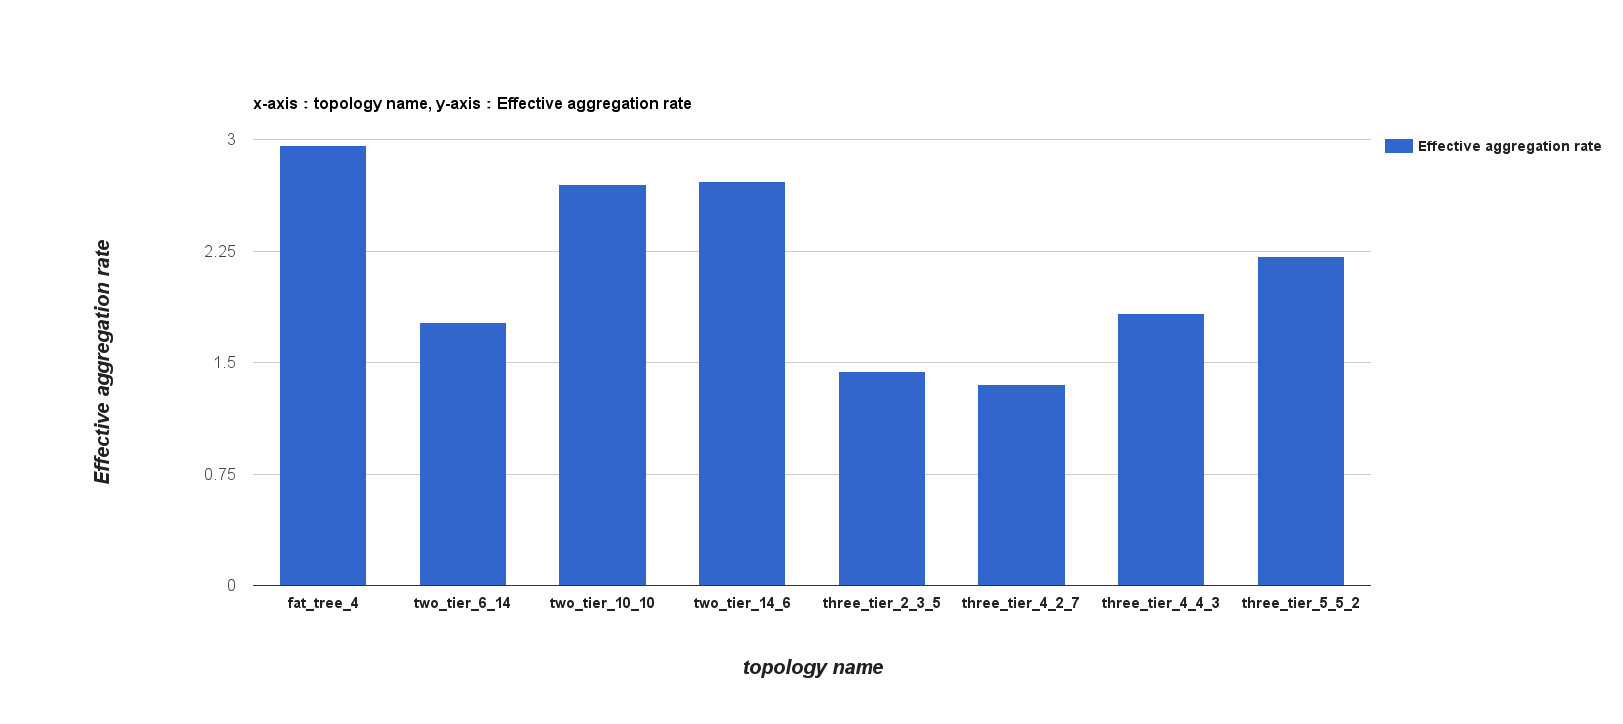
\includegraphics[width=1.4\linewidth]{figures/exp_topotype_bar.png}
\end{center}
\caption{The bar chart of different topologies.}
\label{different_topo_bar}
\end{figure}

From the result in \ref{table:different_topo_type} and Figure~\ref{different_topo_bar}, we can clearly see that although the number of switches are the same, the way how they are connected to each other leads to significant differences. 

And in the 4 three\_tier topologies, the aggregation rates drop as the number of auxiliary entry increases.
We select the most effective one, XXXXXXX, and the least effective one, XXXXXXXX, for further examination with the distribution of the number of entry contained in each group, shown as Figure~\ref{XXXXXXXXXXXX}.



\subsection{Influence of network scale}
XXXXX put different type of topology with roughly the same amount of switch here XXXXX


\begin{comment} XXXXXXXXXXXXXXXXXXXXXXXXXXXXX
As we can see from the trend chart Figure~\ref{XXXXXX}, XXXXXXXXXXXXXX

\begin{figure}[H]
\begin{center} 
\includegraphics[width=1\textwidth]{figures/XXXXXXXXXXXXXXX}
\end{center}
\caption{The trend chart of different.}
\label{flow_entry_detection_flowchart}
\end{figure}
\end{comment}

\subsection{Influence of flow entry number}


In this experiment, we will use only the XXXXXXXXXXXXX and alternate the number of entry on each switch to see the influence it might bring. 
The trend chart Figure ~\ref{XXXXXX} shows that XXXXXXXXXXXXXX
\begin{comment} XXXXXXXXXXXXXXXXXXXXXXXXXXXXX
\begin{figure}[H]
\begin{center} 
\includegraphics[width=1\textwidth]{figures/XXXXXXXXXXXXXXX}
\end{center}
\caption{The flow chart of the flow entry detection process.}
\label{flow_entry_detection_flowchart}
\end{figure}
\end{comment}




-------------------------
However, the aggregation rates do not always grow along with the scale of the network. The reason is that XXXXXXXXXXXXX


link number

the number of host 

strangle 


 